\documentclass[a4paper, 12pt]{article}

\usepackage[italian]{babel}
\usepackage{tikz}
\usepackage{xcolor}
\usepackage{graphicx}
\usepackage{hyperref}
\usepackage{imakeidx}
\usepackage{caption}
\usepackage{fancyhdr}
\usepackage{tabularx}


%--------------------Default Settings--------------------
\def\logo{Immagini/logo.jpeg}% modifico di path
\def\titolo{Lettera di Candidatura}
\def\nomeGruppo{Alt+F4}
%------------------------------------------------

\usetikzlibrary{calc}
\definecolor{fp-blue}{HTML}{2885c8}
\definecolor{fp-red}{HTML}{ea5f64}
\makeindex[title=Indice]
\hypersetup{hidelinks}

\pagestyle{fancy}
\fancyhead[L]{\titolo}
\setlength{\headheight}{15pt}
\fancyhead[R]{\nomeGruppo}
%zero spazio quando vai a capo
\setlength{\parindent}{0pt}

\renewcommand{\familydefault}{\sfdefault}
\newcommand{\glossario}[1]{\fontfamily{lmr}\selectfont{\textit{#1\textsubscript{\small G}}}}

%--------------------INFORMAZIONI PRIMA PAGINA-------------------- 
\title{\Huge \textbf{\titolo}}
\author{\Large{Alt} \raisebox{0.3ex}{\normalsize  +} \Large{F4}}
\date{31 ottobre 2024}
%----------------------------------------------------------------

\begin{document}

\begin{titlepage}      
    \maketitle
    \thispagestyle{empty}  

    \begin{tikzpicture}[remember picture, overlay]
        \fill[fp-blue] 
        ($(current page.south west) + (0, 10)$) 
        -- ($(current page.center) + (0, -8)$)
        -- ($(current page.center) + (0, -15)$)
        -- (current page.south west);

        \fill[fp-red]
        ($(current page.south east) + (0, 10)$) 
        -- ($(current page.center) + (0, -8)$)
        -- ($(current page.center) + (0, -15)$)
        -- (current page.south east);

        \clip ($(current page.center) + (0, -8)$) circle (1cm) node 
        {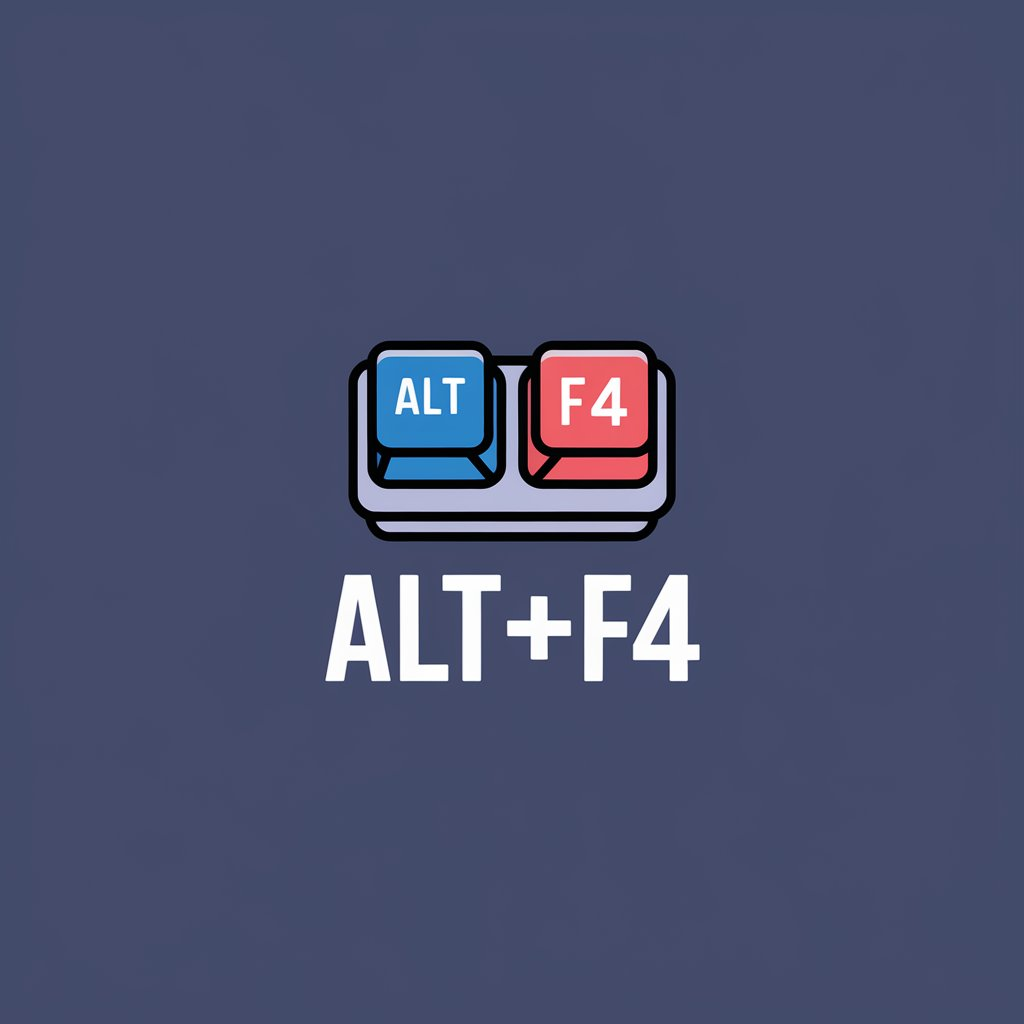
\includegraphics[width=.25\textwidth]{\logo}};
        
    \end{tikzpicture}
\end{titlepage}

\newpage

\textbf{Egregio Professor Vardanega},\\
\textbf{Egregio Professor Cardin}, \\
con la presente, il gruppo Alt+F4 desidera comunicare la propria volontà e decisione di candidarsi per lo sviluppo e la realizzazione del capitolato proposto dall’azienda \textbf{Azzurrodigitale}, denominato \textbf{Buddybot}.\\

La repository relativa alla documentazione è disponibile al seguente indirizzo:\\

\textbf{https://github.com/ALT-F4-eng/Documentazione}\\

In particolare, sono presenti i seguenti documenti:
\begin{itemize}
    \item \textbf{Verbali interni}
    \begin{itemize} % Ambiente itemize annidato
        \item 16 ottobre 2024
        \item 22 ottobre 2024
        \item 28 ottobre 2024
        \item 29 ottobre 2024
    \end{itemize}
    \item \textbf{Verbali esterni}
    \begin{itemize} 
        \item 25 ottobre 2024 - Ergon Infromatica Srl
        \item 25 ottobre 2024 - Azzurrodigitale
        \item 30 ottobre 2024 - Sanmarco Infromatica SPA
    \end{itemize}
    \item \textbf{Valutazione dei capitolati}
    \item \textbf{Preventivo costi e Assunzione impegni}
\end{itemize}
Inoltre, il gruppo si propone di completare la realizzazione entro il:
\textbf{21 aprile 2025}.Come evidenziato nel documento \textit{Preventivo costi e assunzione impegni} il costo complessivo stimato ammonta a: € \textbf{11130}.\\

\newpage

Il gruppo Alt+F4 è composto dai seguenti membri:
\begin{table}[h]
    {\renewcommand{\arraystretch}{2}
    \begin{tabularx}{\textwidth}{| X | X |}
        \hline
            \textbf{\large Nome Cognome} & 
            \textbf{\large Matricola} \\
        \hline 
        \hline
            Enrico Bianchi&
            2040978 \\
        \hline 
            Eghosa Matteo Igbinedion Osamwonyi&
            2042888 \\
        \hline 
            Guirong Lan&
            2042368 \\
        \hline 
            Pedro Leoni&
            2042359 \\
        \hline 
            Marko Peric&
            2011067 \\
        \hline 
            Francesco Savio&
            2085846 \\
        \hline 
    
\end{tabularx}}
\newline
\newline
\newline
\newline
Cordiali saluti,\\
\textit{Alt+F4}.
\end{table}


\end{document}